\documentclass[12pt, letterpaper]{article}
\usepackage[utf8]{inputenc}
\usepackage{graphicx}
\usepackage{amsmath}

\title{Creating a Test Statistic to Find if the Number of Misses in a Song from Guitar Hero is Random}
\author{Shannon Coyle, Samantha Colucci, and Brianna Cirillo}
\date{December 2020}

\begin{document}
\maketitle

\section{INTRODUCTION}
The game, Guitar Hero, collects information regarding the number of “hits” recorded by the player.  This poses the question about the randomness of the misses in a song and if they are correlated to the difficulty of the part of the song.

The study investigates the randomness of different songs using varying methods.  These methods looked at the number of miss streaks over the total number of misses, distances between each miss, and using the runs test.  The resampling of the data sets was performed through parametric bootstrapping, permutation tests, and regular bootstrapping. Using resampling and our methods together allowed us to assess the randomness of a given song based on the results. 

This report explains the methodology used in order to test the randomness of a song. The methods and resampling used throughout the project gave results for the empirical type 1 error and the power of the test. These methods were applied to different songs, therefore, returning different results. This report will also look at the limitations and future ideas for the project, and how some of our methods worked well while others did not.

\section{METHODOLOGY}
\subsection{Method 1}
The first method looks at the proportion of the number of miss streaks over the number of total misses.  A streak was definied as one or more misses in a row since it was easier with the code and some samples did not have that many streaks to look at.  From this method, we discovered that the proportion does not tell us anything about the location of the misses.  This proved to be difficult to determine randomness of misses without knowing the exact location of them.  

\subsection{Method 2}
The second method calculates the distances between misses in a song.  The idea behind this method was that if we can see where the misses are occurring, we can see if they are random.  We can seeing where the distances are occuring randomly and conclude that the misses must also be occurring randomly. 

There was an attempt to use a median distance as a basis rather than the mean because the distances were varied, so the average would not tell us that much.  This led to a problem because a lot of the songs had long miss streaks, which lead to a distance of 0, so the median would also become zero.  With this small issue, it led to the idea of use the runs test on this method and, therefore, the distances.  

\subsection{Runs Test}
Knowing that the runs test is a preconceived test for randomness, the idea behind using this was to use it on the distances of misses within a song, rather than just using it on the song. As mentioned previously if a conclusion can be reached that the distances are random, this would imply randomness of the misses in the song. 

A run is defined as a series of increasing or decreasing values, while the number of values in each series is the length of each run. The number of runs in a data set is crucial because this is the number that is used to derive the test statistic. The other values involved in deriving the test statistics is the exected number of runs, the median value of the data sample, and the number of values below and above the median.

\subsection{Resampling Methods}
\subsubsection{Parametric Bootstrap}
The Parametric Bootstrap was used to generate a bootstrap using a parameterized distribution.  It takes in a specified number of resamples then performs a Bernoulli distribution in order to resample the data.  The Bernoulli distribution looks at the sample size then the event probability, which was set to 50\% since the data is composed of 0's and 1's.  This goes through and resamples the data as either a 0 or a 1 for the specified number of resamples that was initialized.   

\subsubsection{Permutation Tests}
\subsubsection{Regular Bootstrap}


\section{EMPIRICAL TYPE 1 ERROR AND POWER SIMULATIONS}

\subsection{Parametric Bootstrap}
\subsubsection{Empirical Type 1 Error} 

\begin{tabular}{|c|c|}
\textbf{Type 1 Error} & \textbf{Random Song 1}\\
$\alpha = 0.001$ & 0.00\\
$\alpha = 0.005$ &  0.01\\
$\alpha = 0.006$ &  0.01\\
$\alpha = 0.007$ & 0.01\\
$\alpha = 0.008$ & 0.01\\
$\alpha = 0.009$ & 0.01\\
$\alpha = 0.01$ & 0.01\\
$\alpha = 0.02$ & 0.01\\
$\alpha = 0.03$ & 0.01\\
$\alpha = 0.04$ & 0.01\\
$\alpha = 0.05$ &  0.03\\
$\alpha = 0.06$ &  0.06\\
$\alpha = 0.07$ &  0.08\\
$\alpha = 0.08$ &  0.08\\
$\alpha = 0.09$ & 0.08\\
$\alpha = 0.1$ & 0.08 \\
\end{tabular}

\subsubsection{Final Power Simulations}
\begin{tabular}{|c|c|c|c|c|c|}
\hline
\textbf{Type 1 Error Rate Scenario} & $\alpha = 0.001$ &  $\alpha = 0.005$ &  $\alpha = 0.01$ &  $\alpha = 0.05$ &  $\alpha = 0.10$ \\
\hline
Neg. Pair Correlation, n = 200 & 0.00 & 0.00 & 0.00 & 0.00 & 0.00 \\
\hline
Neg. Pair Correlation, n = 600 & 0.00 & 0.00 & 0.00 & 0.00 & 0.00 \\
\hline
Blocks, n = 200 & 0.00 & 0.03 & 0.03 & 0.11 & 0.30 \\
\hline
Blocks, n = 600 & 0.00 & 0.00 & 0.01 & 0.02 & 0.08 \\
\hline
AR(1), p=0.1, $\rho = 0.5$, n = 200 & 0.00 & 0.00 & 0.00 & 0.00 & 0.00 \\
\hline
AR(1), p=0.1, $\rho = 0.5$, n = 600 & 0.00 & 0.00 & 0.00 & 0.00 & 0.00 \\
\hline
AR(1), p=0.1, $\rho = 0.3$, n = 200 & 0.00 & 0.00 & 0.00 & 0.01 & 0.01 \\
\hline
AR(1), p=0.1, $\rho = 0.3$, n = 600 & 0.00 & 0.00 & 0.00 & 0.00 & 0.00 \\
\hline
AR(1), p=0.2, $\rho = 0.5$, n = 200 & 0.00 & 0.00 & 0.00 & 0.00 & 0.00 \\
\hline
AR(1), p=0.2, $\rho = 0.5$, n = 600 & 0.00 & 0.00 & 0.00 & 0.00 & 0.00 \\
\hline
\end{tabular}

\subsection{Permutation Test}
\subsection{Regular Bootstrap}


\section{APPLICATION}
To obtain a p-value for each song, 100 bootstraps were performed to change the 0's and 1's to different orders and sequences.  Previously, 1000 bootstraps were being done, but it was taking a significant amount of time to return a p-value.  The null hypothesis being followed is that the songs are random and the alternative hypothesis is that the songs are not random. 

\subsection{Song 1: "Judith"}

\subsubsection{Parametric Bootstrap}
\begin{tabular}{|c|c|c|}
\hline
\textbf{Method Type} & P-Value \\
\hline
Method 1 & 0 \\
\hline
Runs Test & 0.512 \\ 
\hline
\end{tabular}


\subsubsection{Permutation Tests}
\subsubsection{Regular Bootstrap}

\subsection{Song 2: "Hurts"}

\subsubsection{Parametric Bootstrap}
\begin{tabular}{|c|c|c|}
\hline
\textbf{Method Type} & P-Value \\
\hline
Method 1 & 0  \\
\hline
Runs Test & 0.512 \\ 
\hline
\end{tabular}

\subsection{Song 3: "American Girl"}
\subsubsection{Parametric Bootstrap}

\begin{tabular}{|c|c|}
\hline
\textbf{Method Type} & P-Value \\
\hline
Method 1 & 0.16 \\
\hline
Runs Test & 0.211 \\ 
\hline 
\end{tabular}

\subsection{Song 4: "Funky"}
\subsubsection{Parametric Bootstrap}

\begin{tabular}{|c|c|c|}
\hline
\textbf{Method Type} & P-Value \\
\hline
Method 1 & 0 \\
\hline
Runs Test & 0.08  \\ 
\hline
\end{tabular}

\subsection{Song 5: "Ring of Fire"}
\subsubsection{Parametric Bootstrap}

\begin{tabular}{|c|c|c|}
\hline
\textbf{Method Type} & P-Value  \\
\hline
Method 1 & 2.204 $[e^{-16}]$ \\
\hline
Runs Test & 0.44 \\ 
\hline
\end{tabular}

\subsection{Song 6: "Watchtower"}
\subsubsection{Parametric Bootstrap}

\begin{tabular}{|c|c|c|}
\hline
\textbf{Method Type} & P-Value  \\
\hline
Method 1 & 2.204 $[e^{-16}]$ \\
\hline
Runs Test & 0.66 \\ 
\hline
\end{tabular}
\subsection{Song 7: "Wolf"}
\subsubsection{Parametric Bootstrap}

\begin{tabular}{|c|c|c|}
\hline
\textbf{Method Type} & P-Value  \\
\hline
Method 1 & 2.204 $[e^{-16}]$ \\
\hline
Runs Test & 0.58 \\ 
\hline
\end{tabular}


\section{DISCUSSION/LIMITATIONS/IDEAS FOR FURTHER RESEARCH}


\section{APPENDIX}
\begin{figure}
\centering
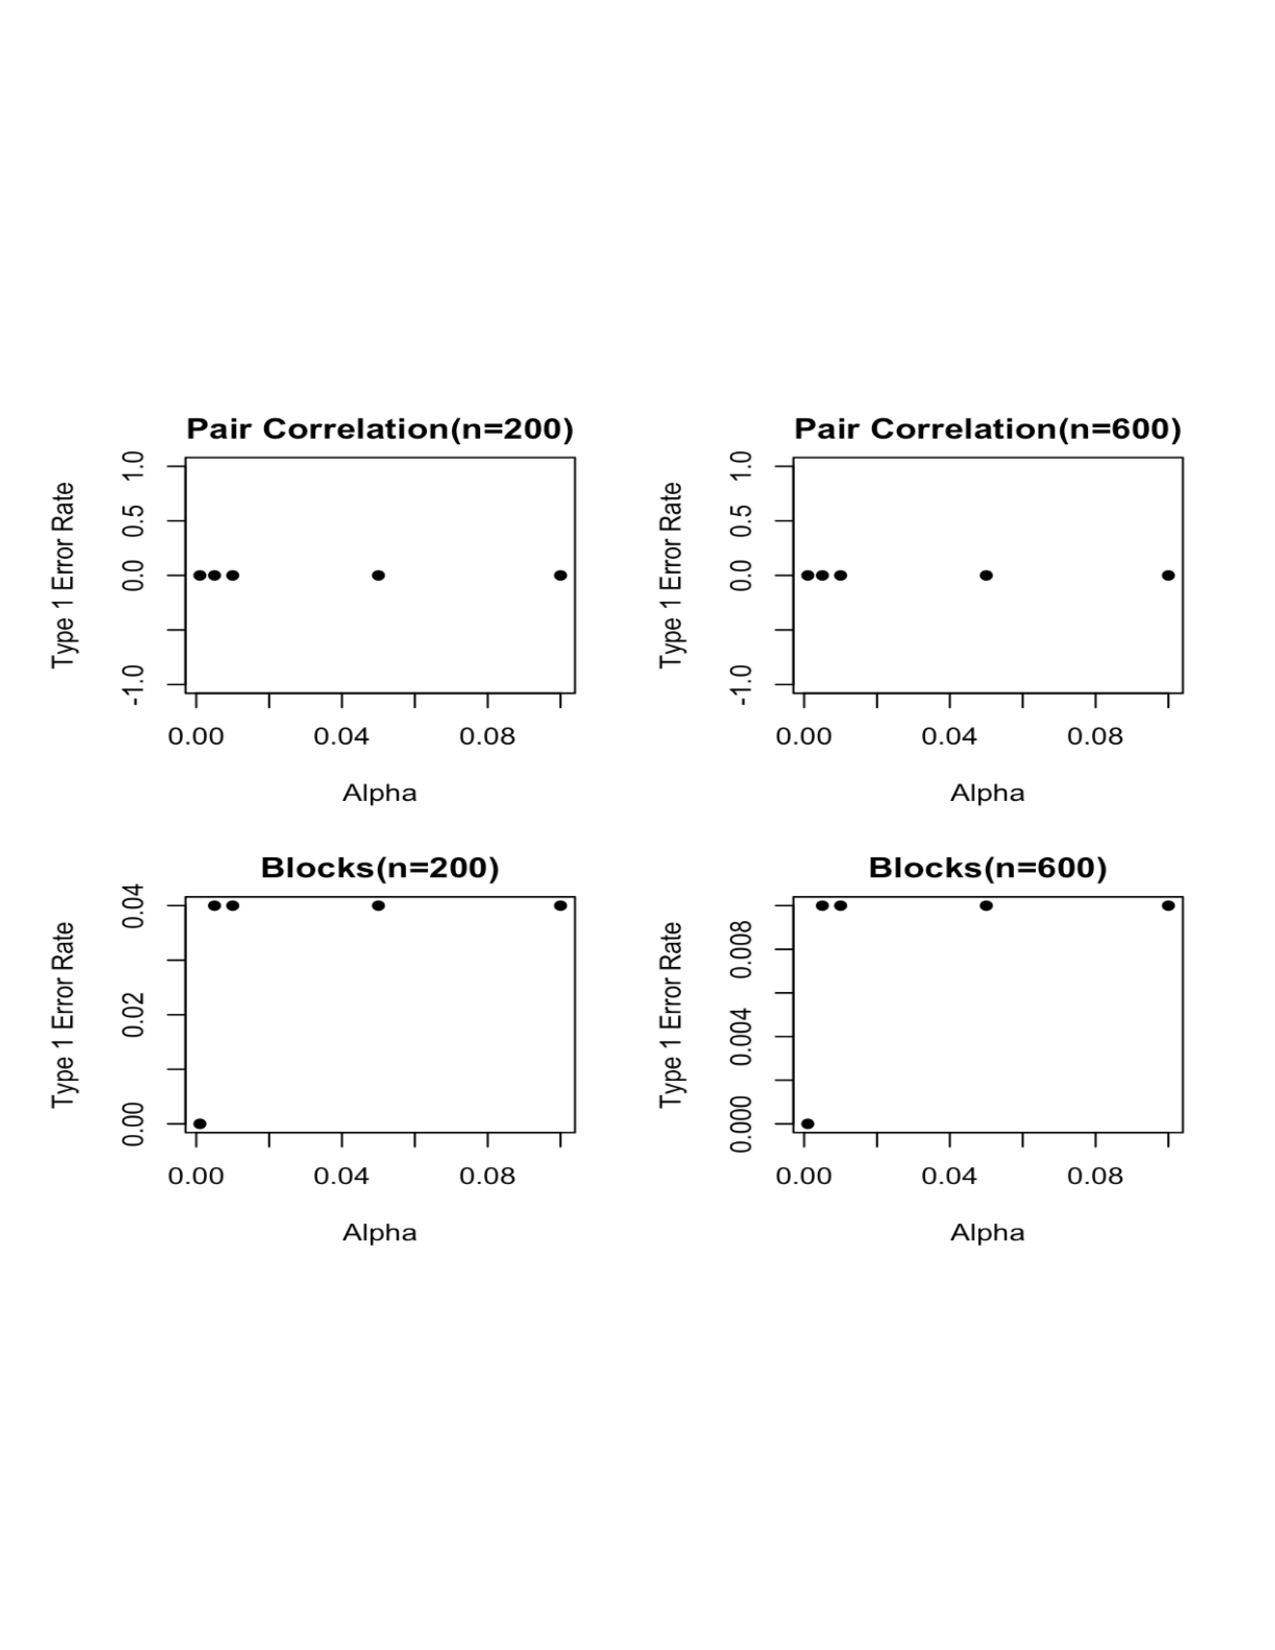
\includegraphics[width=7cm]{Pari Correlation.pdf}
\caption{Pairwise Correlation}
\label{fig: Pair Correlation Plot}
\end{figure}

\section{PERSONAL REFLECTIONS}
\subsection{Brianna Cirillo}
\subsection{Samantha Colucci}
\subsection{Shannon Coyle}


\end{document}